\documentclass[conference]{IEEEtran}
\IEEEoverridecommandlockouts
% The preceding line is only needed to identify funding in the first footnote. If that is unneeded, please comment it out.
\usepackage{cite}
\usepackage{float}
\usepackage{amsmath,amssymb,amsfonts}
\usepackage{algorithmic}
\usepackage{graphicx}
\usepackage{textcomp}
\usepackage{subfig}
\usepackage{fixltx2e}
\usepackage{stfloats}
\def\BibTeX{{\rm B\kern-.05em{\sc i\kern-.025em b}\kern-.08em
    T\kern-.1667em\lower.7ex\hbox{E}\kern-.125emX}}
\begin{document}

\title{Exploiting Path Diversity in Datacenters using MPTCP-aware SDN}

\author{\IEEEauthorblockN{Bc. Tomas Urban}
\IEEEauthorblockA{\textit{Faculty of Informatics and Information Technologies}\\
\textit{Slovak Technical University in Bratislava}\\
Bratislava, Slovakia \\
xurbant@stuba.sk}
\and
\IEEEauthorblockN{Bc. Martin Oravsky}
\IEEEauthorblockA{\textit{Faculty of Informatics and Information Technologies}\\
\textit{Slovak Technical University in Bratislava}\\
Bratislava, Slovakia \\
xoravskym@stuba.sk}

}

\maketitle

\begin{abstract}
Multipath TCP (MPTCP) has been proposed as an alternative transport approach mainly for datacenter networks. MPTCP provides the ability to split a flow into multiple paths providing better performance and resilience to failures. MPTCP is combined with flow-based Equal-Cost Multi-Path Routing (ECMP), which uses random hashing to split the MPTCP subflows over different paths. Random hashing can be suboptimal as distinct subflows may end up using the same paths, while other available paths remain unutilized. In our solution we create an MPTCP-aware SDN controller that facilitates an alternative routing mechanism for the MPTCP subflows. Our controller uses packet inspection providing deterministic assignment of subflows. Using this approach we demonstrate better performance while there is no limitation regarding access links of particular hosts. We also investigate the usage of multiple interfaces at the hosts in order to eliminate limitation of throughput due to access links.
\end{abstract}

\begin{IEEEkeywords}
mptcp, multipath, sdn, controller, subflow, ecmp
\end{IEEEkeywords}

\section{Introduction}
~\indent The Transmission Control Protocol (TCP) is used by the vast majority of applications
to transport their data reliably across the Internet. TCP was designed in
the 1970s, and neither mobile devices nor computers with many network interfaces
were an immediate design priority. On the other hand, the TCP designers
knew that network links could fail, and they chose to decouple the network-layer
protocols (Internet Protocol) from those of the transport layer (TCP) so that the
network could reroute packets around failures without affecting TCP connections.
This ability to reroute packets is largely due to the use of dynamic routing protocols,
and their job is made much easier because they don�t need to know anything
about transport-layer connections.

\indent Today�s networks can be multipath: mobile devices have multiple wireless interfaces,
datacenters have many redundant paths between servers, and multihoming has
become the norm for big server farms. Meanwhile, TCP is essentially a single-path
protocol: when a TCP connection is established, the connection is bound to the IP
addresses of the two communicating hosts. If one of these addresses changes, for
whatever reason, the connection will fail. In fact, a TCP connection cannot even be
load balanced across more than one path within the network, because this results
in packet reordering, and TCP misinterprets this reordering as congestion and
slows down.

\indent This mismatch between today�s multipath networks and TCP�s single-path design
creates tangible problems. For instance, if a smartphone�s WiFi loses signal, the
TCP connections associated with it stall; there is no way to migrate them to other
working interfaces, such as 3G. This makes mobility a frustrating experience for
users. Modern datacenters are another example: many paths are available between
two endpoints, and multipath routing randomly picks one for a particular TCP
connection. This can cause collisions where multiple flows get placed on the same
link, thus hurting throughput to such an extent that average throughput is halved
in some scenarios.

\indent Multipath TCP (MPTCP)\cite{1} \cite{7} is a major modification to TCP that allows multiple
paths to be used simultaneously by a single transport connection. Multipath
TCP circumvents the issues mentioned above and several others that affect TCP.
Changing TCP to use multiple paths is not a new idea; it was originally proposed
more than 15 years ago by Christian Huitema in the Internet Engineering Task
Force (IETF), and there have been a half-dozen more proposals since then to
similar effect. Multipath TCP draws on the experience gathered in previous work,
and goes further to solve issues of fairness when competing with regular TCP and
deployment issues as a result of middleboxes in today�s Internet. The Multipath
TCP protocol has recently been standardized by the IETF, and an implementation
in the Linux kernel is available today\cite{2}.

\section{Analysis}
\subsection{Chapter introduction}

~\indent This chapter is a brief analysis of Software defined networking and how it can
benefit from multipath transmission control protocols, especially in datacenter-like
topologies by exploiting path diversity.

\indent In chapter \ref{analysis:sdn}, the basic concept of software defined networking will be
introduced. Chapter \ref{analysis:mptcp} will briefly talk about Multipath TCP protocol which will be used later in this document. Chapter \ref{analysis:problems} will consider several problems regarding poor performance of SDNs due to random path selection. 

\subsection{Software defined networking}
\label{analysis:sdn}

~\indent Today�s networks mainly consist of routers, switches, hosts and many other network devices. In order for hosts to communicate, routers and switches performs as a transfer point between source and destination. These devices must provide very fast and reliable transfer of information, which, since the need for fast Internet connection is bigger and bigger every year, can be challenging.

\indent The basic network device consists of data plane and control plane. Data plane is responsible for receiving the incoming packet and forwarding it to device�s control plane, where the packet is processed. Control plane then forwards the packet again to the data plane, which then sends the packet via correct outgoing interface. This causes network device to store a lot of information and the CPU load can become quite high.

\indent �Software defined networking is an architectural approach that optimizes and simplifies network operation by more closely binding the interaction (i.e., provosioning, messaging and alarming) among applications and network services and devices, whether they be real or virtualized. �\cite{Nadeau}

\indent SDNs use centralized object known as controller, which does all the computing
and routing of the communication. The controller installs various forwarding rules based on global view of network topology on forwarders. Forwarders (also known as switches) are simple devices which forward the communication based on the rules installed by controller. If packet arrives on forwarder interface and no rule is matched, forwarder sends the packet to controller using OpenFlow protocol. The controller then processes the packet (e.g. flooding ARP request) and sends the packet back to forwarders along with corresponding rule. 

\indent This enables the network to better handle the communication while using the hardware resources better. 


\subsection{Multipath TCP}
\label{analysis:mptcp}

~\indent There are several options when sending communication on multiple path simultaneously while providing better redundancy and throughput. One can use Stream control transmission protocol (SCTP) which uses the concept of streams. When there is a need for L2 redundancy, bonding has proven itself as a good alternative.

\indent In this document we propose Multipath TCP as a great alternative for improving path diversity in multipath communication in datacenter-like topologies.

\indent Multipath TCP utilizes one TCP connection on multiple paths, on which separate TCP subflows are created, thus providing improved throughput and redundancy. Multipath TCP eliminates single point of failure by ability to switch communication to a working path when another path goes down. Multipath TCP enabled hosts use Multipath TCP options to establish a connection or to add a new subflow to an existing connection. 

\subsection{Problems with Multipath TCP and SDNs}
\label{analysis:problems}
~\indent Software defined networking can greatly benefit from Multipath TCP
capabilities. However, software defined networks do not handle MPTCP traffic
differently than the classic single-path TCP traffic. In order to exploit path diversity
better and to provide true redundancy to the network, further implementation on the
controller is necessary.

\indent �A key aspect that affects MPTCP performance is the routing mechanism of
the subflows. Currently, the most prominent and widely deployed routing mechanism
in datacenters is a flow-based variant of Equal-Cost Multi-Path Routing (ECMP)� [2].
However, ECMP uses random hashing to split the subflows over different paths. This
can cause a variety of problems, from which the most important is the high probability
that multiple subflows end up on the same path while other paths remain not utilized
properly. This also destroys the idea of redundancy.

\indent The number of subflows is also a crucial aspect to performance of the network.
Although the idea of more subflows can mean faster networks, the more subflows
MPTCP use, the bigger the overhead is. More subflows mean more rules installed in
forwarders and higher CPU utilization for the controller.

\indent As shown in previous papers, MPTCP throughput also correlates with number
of used interfaces on hosts. We will also deal with this issue since one-homed devices
can quickly become a bottleneck in this type of network.

\indent The purpose of this assessment is to implement an intelligent routing protocol
that makes software defined networks MPTCP-aware by exploiting path diversity. 

\section{Design}
\subsection{Topology}
~\indent The right choice of topology is crucial for datacenter network performance. One of the most used datacenter network topology is FatTree topology, which is shown below on picture 1. The topology consists of pods, which are connected on multiple core switches. The higher the level, the faster the bandwidth.

\begin{figure}[h]
\centerline{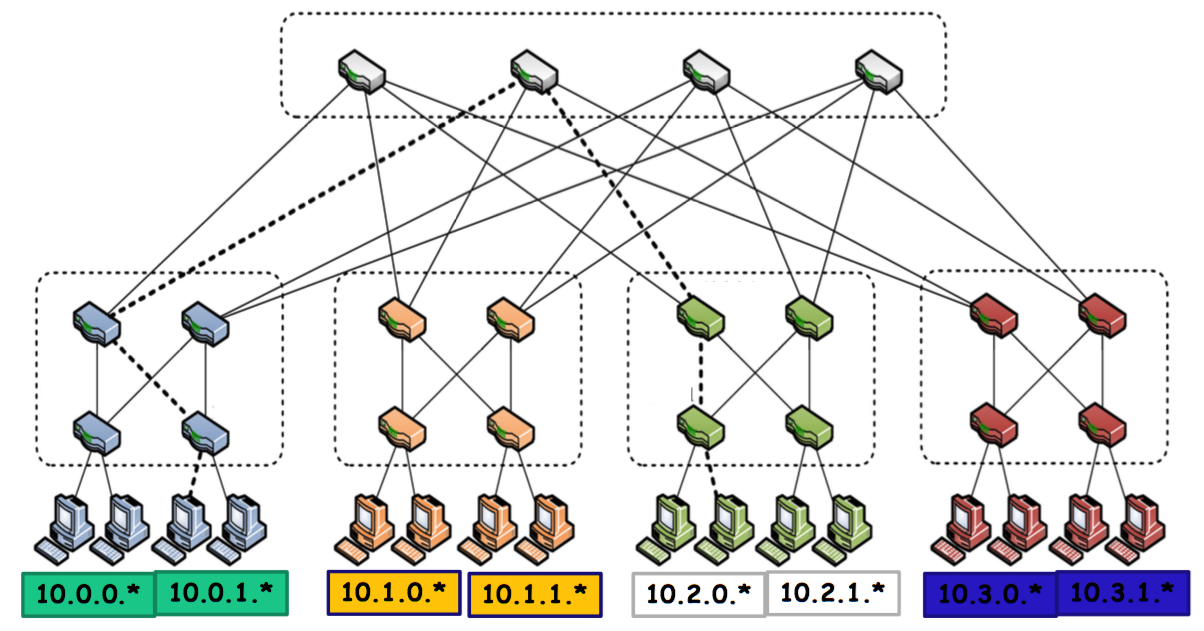
\includegraphics[width=7cm]{fattree}}
\caption{Fattree topology}
\label{fig:fattree}
\end{figure}

\subsection{Controller}

~\indent To make SDN MPTCP-aware, it is necessary to let controller know that multipath communication occurs in the network. This can be achieved by packet inspection on controller. When a packet arrives on a forwarder and no rule is matched, the packet is sent to SDN controller which calculates the path for the subflow by using its global view of the topology. SDN controller then installs the rules onto every single forwarder that lies on the chosen path. The implementation will use Floodlight controller written in Java.

\indent The shortest paths available will be computed using a graph traversal algorithm. Sets of paths will be stored on controller and these will be deterministically assigned to subflows. While using multiple redundant paths, MPTCP�s performance should be maximized using a small number of subflows. Each path should be assigned to only one subflow, this can be achieved by storing IP addresses to paths.

\indent When a new packet arrives on the controller, it will extract the needed information from the packet (IPs, ports, MPTCP options). If the option says we are dealing with a new subflow (MP\_CAPABLE), it will find the shortest path between IPs and store the path into a hashtable. This path is then assigned to a subflow. If the options says we are dealing with additional subflow (MP\_JOIN), we extract the token from the packet and find another shortest path for the subflow. The rules are installed on all switches belonging to the chosen path.

\subsection{Testbed}
~\indent To properly evaluate the algorithm, a virtual testbed will be needed. The tests will be performed on a Linux virtual machine running Floodlight controller and Mininet emulator. We create two more Linux virtual machines with multiple interfaces that will be connected to ports on the switches emulated in Mininet. After running FatTree topology in Mininet, we will evaluate how many subflows are needed in order to maximize MPTCP performance. We will then compare this approach to random approach used by ECMP protocol. 

\section{System overview}
\subsection{Topology}
~\indent In our implementation, various topologies were used. To prove our implementation, we started with very simple one switch topology with two Linux virtual machines as hosts. Each host is connected to the switch using two links. 

\subsubsection{Four-switches topology}

\indent To better evaluate our implementation, we needed to use a topology which enabled hosts to communicate over multiple paths simultaneously. We used topology with a total of four switches which created four different paths between two hosts.

\begin{figure}[h]
\centerline{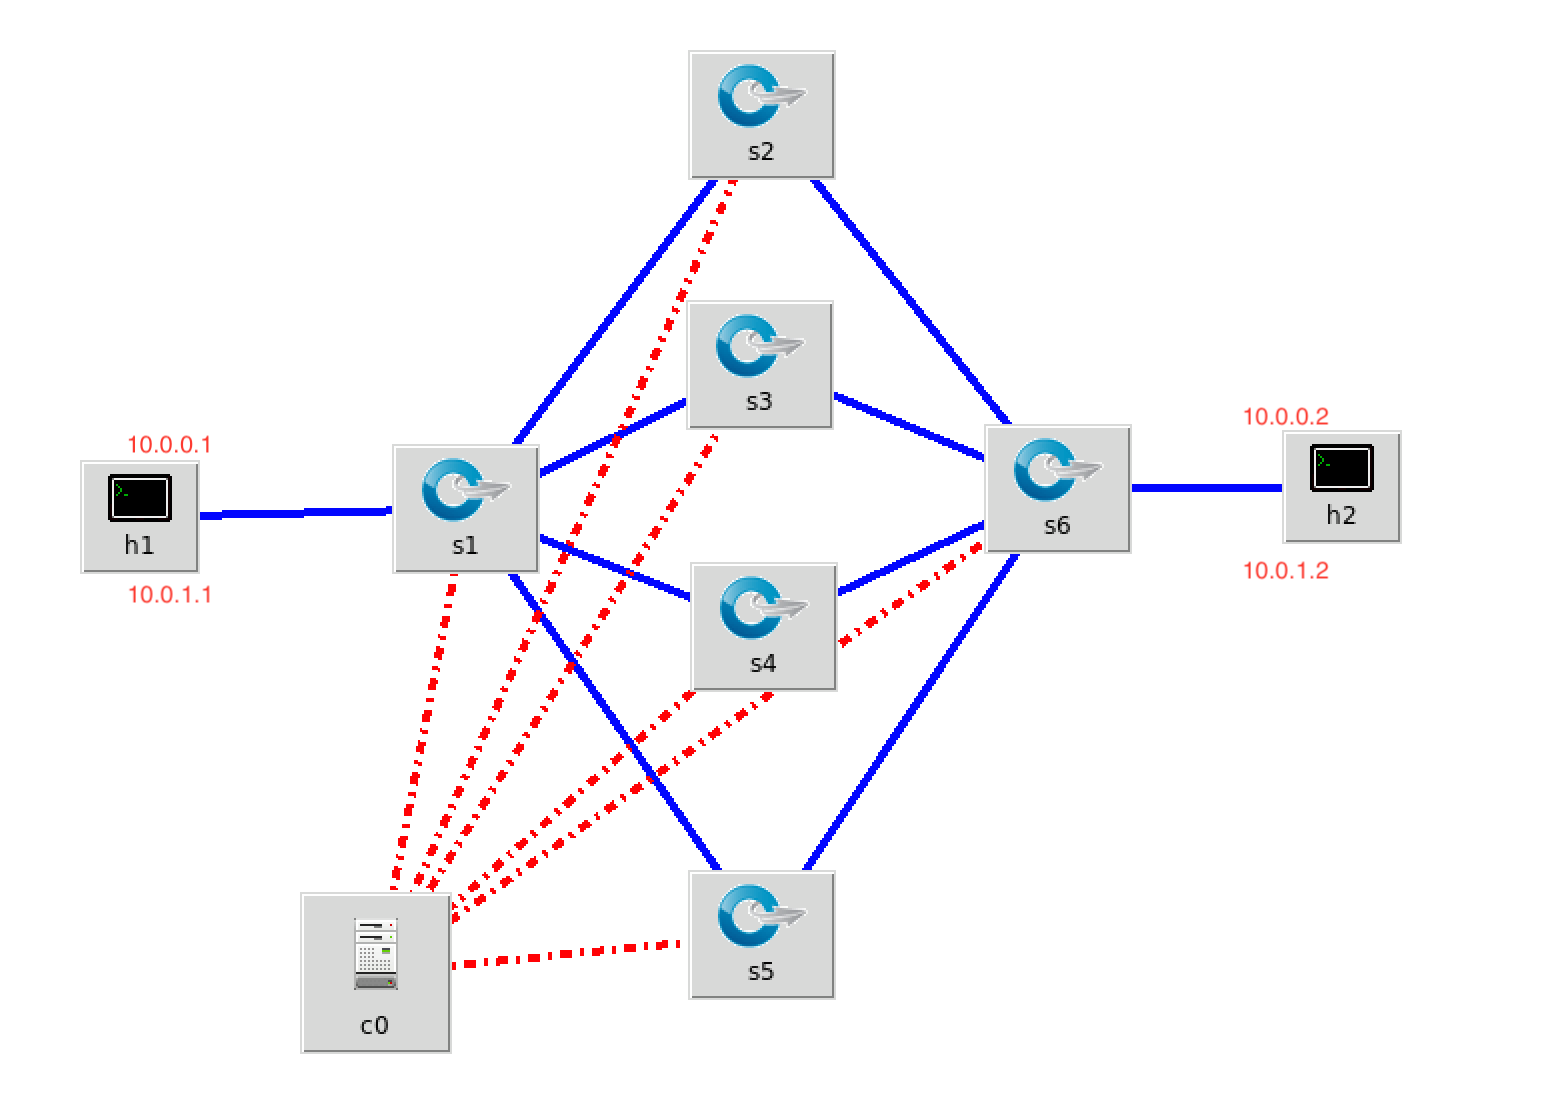
\includegraphics[width=8cm]{4switch}}
\caption{Testing on topology with four switches}
\label{fig:4switch}
\end{figure}


\subsubsection{Controller}
~\indent We have based our controller implementation on RYU controller programmed in Python. The controller has a global view of the network thanks to LLDP exchange during initial switch connection. 

\indent Pre-routing procedures of the controller are described in following sentences. When the controller starts, it flushes all database tables from previous connections. It then adds hosts to the topology. After this procedure, controller uses LLDP packets to obtain a global view of the network topology. Controller also installs a rule that tells switches to forward all TCP communication to the controller. 

\indent The algorithm of routing mechanism is described in following paragraph. 

\indent When SYN packet arrives on the switch, it sends it to the controller. Controller parses MPTCP options, IP addresses, TCP ports and every single value contained in the MPTCP options. This information is then stored into conn, which is a MySQL table used for storing MPTCP connections. 

\indent Controller now installs two rules to the forwarder: one rule for source-destination communication and one for destination-sources communication. Both these rules tell the forwarder to send the communication with mentioned IPs and ports to the controller. 

\indent When SYN-ACK arrives on the controller, our controller parses the needed information and stores it into MySQL database again. 

\indent When ACK arrives on the controller, it calculates every single possible path between source and destination node and then randomly chooses one of them. This prevents single point of failure in the network and better path diversity in the network. Controller then sends a FLOW\_MOD packet to all switches on the selected path send communication out of the proper port. This prevents further communication forwarding to the controller, since it is not needed anymore. 

\indent When joining a new subflow to the connection, the process is very similar to initiating the connection.

\indent The only difference is in the processing of the MP\_JOIN ACK packet, since further actions are needed in order to map subflows to the connection. 

\indent Controller calculates the hash for the subflow and compares it to the hash included in the MP\_JOIN ACK packet. If the hashes are the same, subflows are authenticated and joined to the connection. 

\section{Evaluation}

	\subsection{Setup}
	 ~\indent For our evaluation we used the Mininet emulator 2.2.2 installed on the same machine that is running our controller. It is possible to run Mininet on different machine than controller, although few changes to the implementation are needed. On the machine that runs our controller also run OpenvSwitch 2.5.
	
	\indent Both communicating endpoints were Linux virtual machines running Kernel 4.9 with MPTCP kernel implementation. MPTCP kernel also ran on Controller machine, although this was not necessary. Both host machines had two interfaces connected to our controller machine using virtual internal networks. 

	
		\subsubsection{Topology}
		 \indent We evaluated our implementation on smaller topologies described previously in this paper. Evaluation on bigger datacenter topologies like Fattree or Jellyfish can be evaluted later.

		\subsubsection{Experiments}
		 \indent Our implementation was tested using iperf network program, that creates communication between hosts and can also limit bandwidth of the communication, create parallel TCP communications, etc. 
		
		\indent We ran iperf in server mode on Host2 and connected to it from iperf ran in client mode on Host1. We tested our implementation while also limiting the communication speed.

	
	\subsection{Tests}
	\indent In order to test our algorithm, we executed five different kinds of tests. Following tests were executed:
	
	\begin{enumerate}
	\item Utilization of different paths using 1 subflow between two hosts - deterministic test vs. shortest path forwarding test.
	\item Utilization of different paths using 2 subflows between two hosts - deterministic test vs. shortest path forwarding test.
	\item Average throughput using 4 concurrent connections - deterministic test vs. shortest path forwarding test.
	\item Percentage ratio of worst throughput vs. average throughput using 5 concurrent connections - deterministic test vs. shortest path forwarding test.
	\item Download of file with 100MB file size - deterministic vs. shortest path forwarding.
	\end{enumerate}

	
	\subsection{Results}
	\indent In following subsection we present results of our test with brief sumarization.
	
		%\subsubsection{Utilization of paths - 1 subflow and 2 subflows}
		\begin{figure}[!h]
		\centering
		\subfloat[]{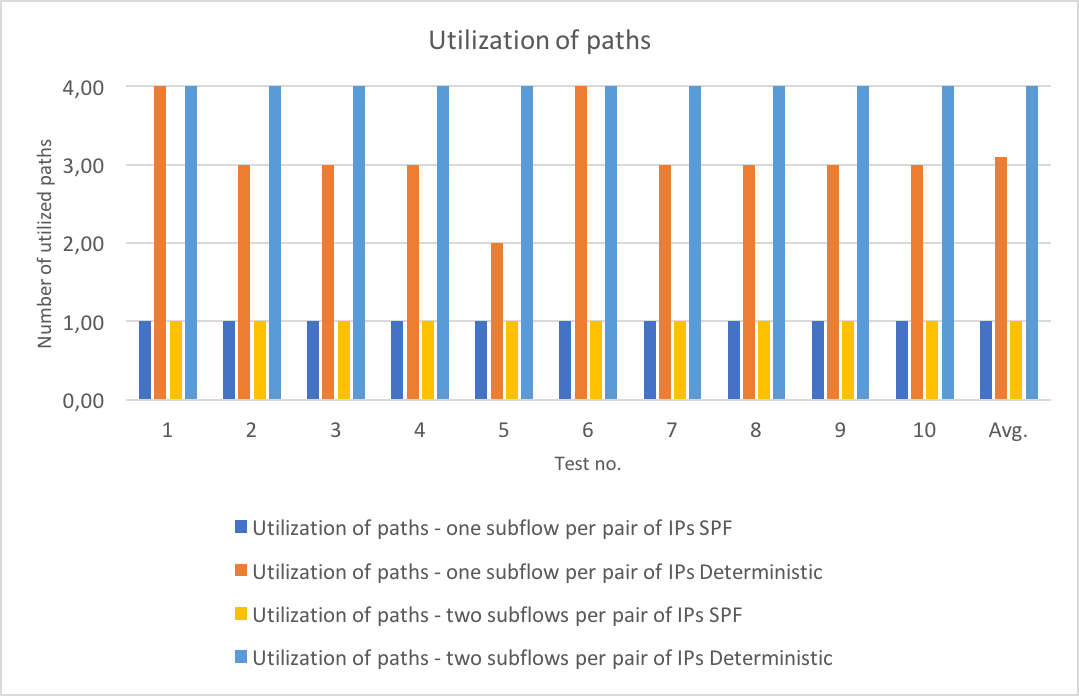
\includegraphics[width=8cm]{graph12}} \hfill
		\caption{Utilization of different paths using 1 and 2 subflows between two hosts - deterministic test vs. SPF test.}
		\label{fig:graph12}
		\end{figure}
		
		\indent MPTCP kernel implementation enables us to use more than one subflow between one pair of IP addresses. For example, when creating fullmesh subflows between two hosts with two interfaces and two subflows per IP pair, a total of 8 subflows will be created. In our tests we compared bandwidth when using one and two subflows between one pair of IP addresses. We did not see any throughput improvement when using more than two subflows per one IP pair probably due to massive packet reordering. Graph \ref{fig:graph12} shows results of these tests. As we can see, on average 3.1 paths were utilized when using deterministic subflow routing. Shortest path forwarding only used one path, since it always chose one shortest path. While using two subflows per pair of IP address we were able to improve path utilization even better. In every experiment deterministic subflow routing utilised every single path available while creating better path redundancy and slightly improving network throughput. Shortest path forwarding still performed poorly as it only created one path. 
				
	%\subsubsection{Average throughput - 4 concurrent connections}
		\begin{figure}[!h]
		\centering
		\subfloat[]{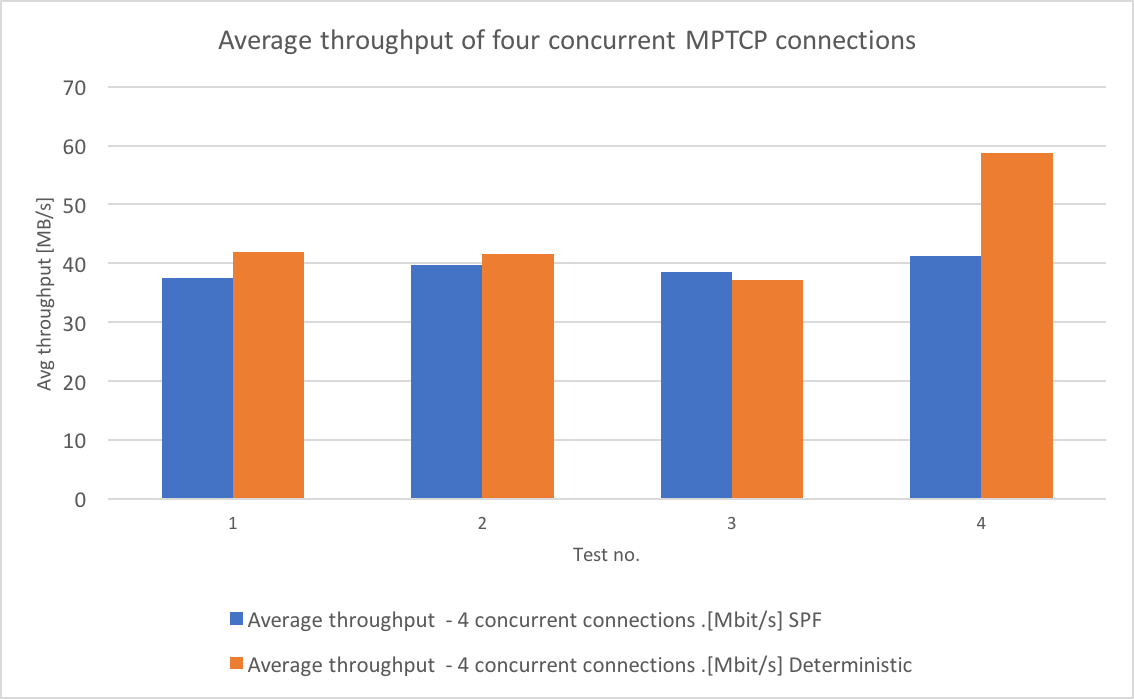
\includegraphics[width=8cm]{graph3}} \hfill
		\caption{figure}{Average throughput using 4 concurrent connections - deterministic test vs. SPF test.}
		\label{fig:graph3}
		\end{figure}
		\indent This test was performed using 4 concurrent MPTCP connections between client and server. Same experiment was executed for 4 times and the average throughtput was calculated for deterministic tests as well as for SPF test. Graph \ref{fig:graph3} shows these values. In this tests, SPF test was slightly outperformed by deterministic test.
			
		%\subsubsection{Download of 100MB file}	
		\begin{figure}[!h]
		\centering
		\subfloat[]{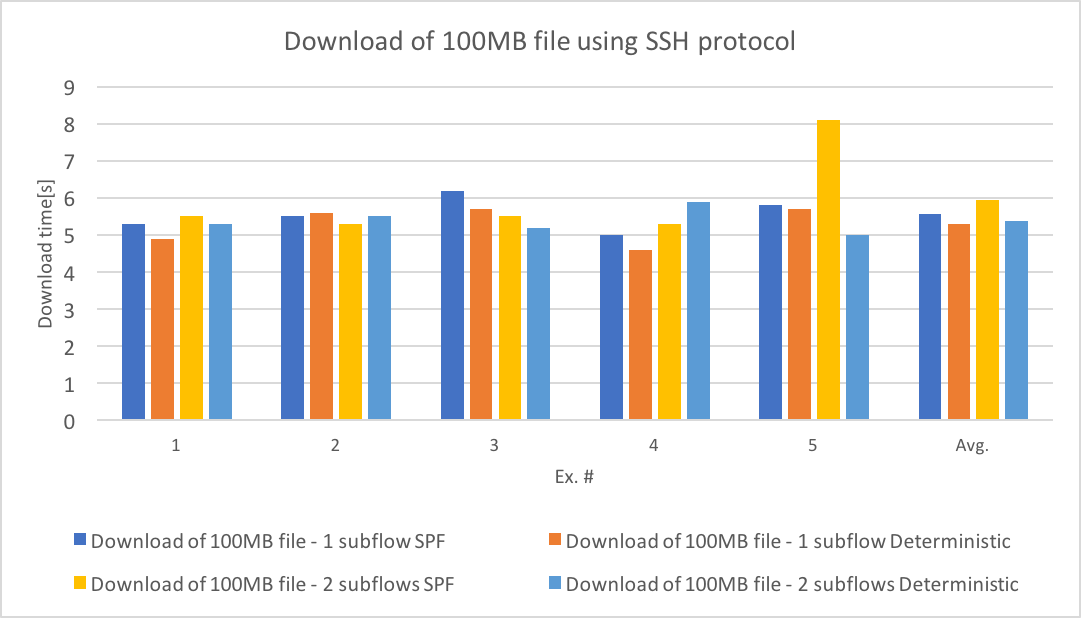
\includegraphics[width=8cm]{graph5}} \hfill
		\caption{Time spent to download 100MB file - deterministic vs. SPF}
		\label{fig:graph5}
		\end{figure}
		
		\begin{figure}[!h]
		\centering
		\subfloat[]{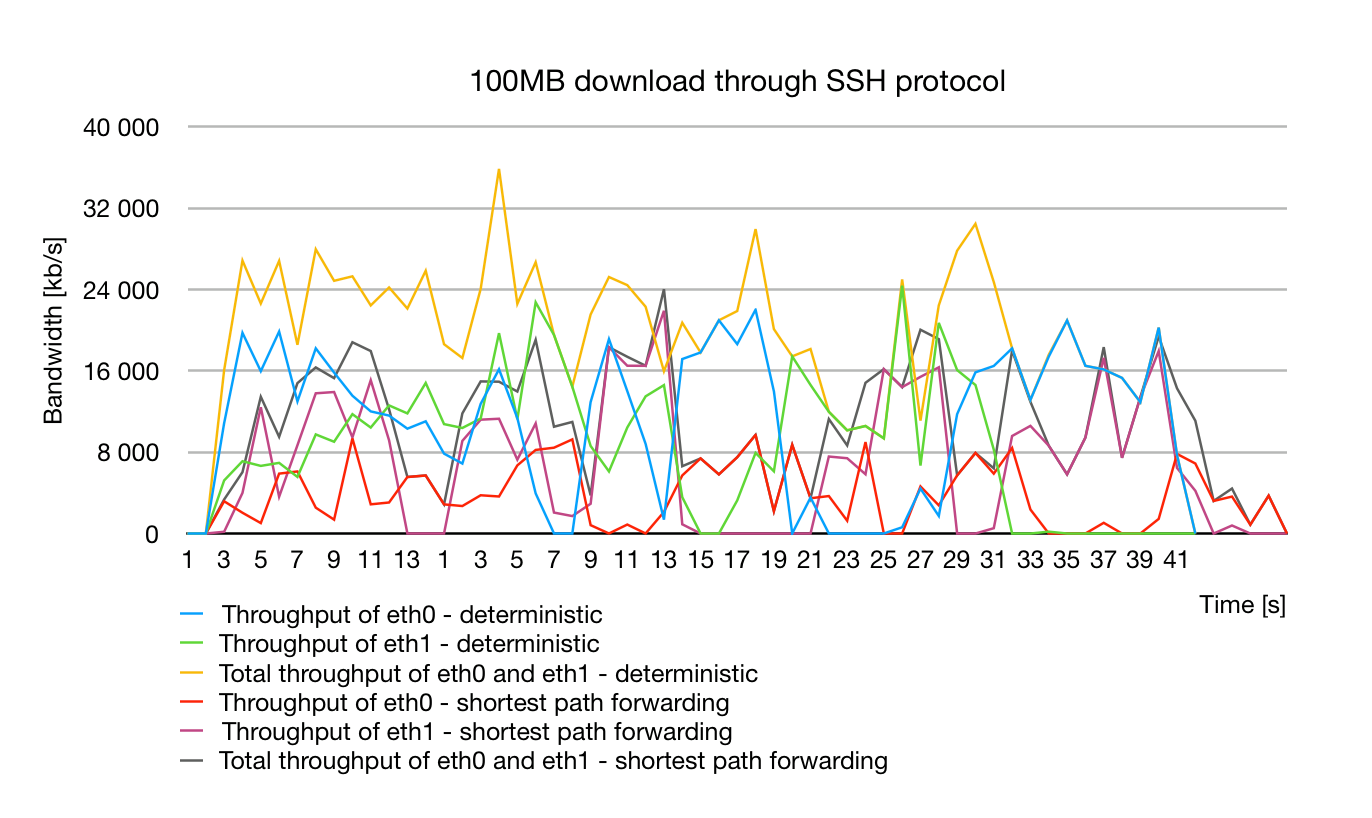
\includegraphics[width=8cm]{graph6}} \hfill
		\caption{Bandwidth during 100MB file download - deterministic vs. SPF.}
		\end{figure}
			
		%\subsubsection{Worst vs. average throughput}
		%\begin{figure}[!h]
		\indent During our tests we also compared worst throughput of conncurrent connections with average throughput. 
				
		\indent Both approaches to routing multipath traffic were tested 3 three times. SPF approach surprisingly performed much better than our deterministic approach. The throughputs were very similar in both approaches, however, in shortest path forwarding approach, each test performed very similar, thus creating very small difference between worst throughput and average throughput. 
				
		\indent In deterministic approach, worst throughput was approximately 75\% of average throughput, whereas worst throughput in SPF approach was at least 92\% of average throughput.
		%\end{figure}
	


\section{Conclusion}
\indent Lorem ipsum


\bibliographystyle{IEEEtran}
\bibliography{bibfile}

\end{document}
